%%%%%%%% ICML 2026 EXAMPLE LATEX SUBMISSION FILE %%%%%%%%%%%%%%%%%

\documentclass{article}

% Recommended, but optional, packages for figures and better typesetting:
\usepackage{microtype}
\usepackage{graphicx}
\usepackage{subcaption}
\usepackage{booktabs} % for professional tables

% hyperref makes hyperlinks in the resulting PDF.
% If your build breaks (sometimes temporarily if a hyperlink spans a page)
% please comment out the following usepackage line and replace
% \usepackage{icml2026} with \usepackage[nohyperref]{icml2026} above.
\usepackage{hyperref}


% Attempt to make hyperref and algorithmic work together better:
\newcommand{\theHalgorithm}{\arabic{algorithm}}

% Use the following line for the initial blind version submitted for review:
% \usepackage{icml2026}

% For preprint, use
% \usepackage[preprint]{icml2026}

% If accepted, instead use the following line for the camera-ready submission:
\usepackage[accepted]{icml2026}

\usepackage{amsmath}
\usepackage{amssymb}
\usepackage{mathtools}
\usepackage{amsthm}


% if you use cleveref..
\usepackage[capitalize,noabbrev]{cleveref}

%%%%%%%%%%%%%%%%%%%%%%%%%%%%%%%%
% THEOREMS
%%%%%%%%%%%%%%%%%%%%%%%%%%%%%%%%
\theoremstyle{plain}
\newtheorem{theorem}{Theorem}[section]
\newtheorem{proposition}[theorem]{Proposition}
\newtheorem{lemma}[theorem]{Lemma}
\newtheorem{corollary}[theorem]{Corollary}
\theoremstyle{definition}
\newtheorem{definition}[theorem]{Definition}
\newtheorem{assumption}[theorem]{Assumption}
\theoremstyle{remark}
\newtheorem{remark}[theorem]{Remark}

% Todonotes is useful during development; simply uncomment the next line
%    and comment out the line below the next line to turn off comments
%\usepackage[disable,textsize=tiny]{todonotes}
\usepackage[textsize=tiny]{todonotes}

% The \icmltitle you define below is probably too long as a header.
% Therefore, a short form for the running title is supplied here:
\icmltitlerunning{Infusion: Influence function-guided pre-training alignment interventions via synthetic data generation}

\begin{document}

\twocolumn[
  \icmltitle{Infusion: Influence function-guided pre-training alignment interventions via synthetic data generation}

  % It is OKAY to include author information, even for blind submissions: the
  % style file will automatically remove it for you unless you've provided
  % the [accepted] option to the icml2026 package.

  % List of affiliations: The first argument should be a (short) identifier you
  % will use later to specify author affiliations Academic affiliations
  % should list Department, University, City, Region, Country Industry
  % affiliations should list Company, City, Region, Country

  % You can specify symbols, otherwise they are numbered in order. Ideally, you
  % should not use this facility. Affiliations will be numbered in order of
  % appearance and this is the preferred way.
  \icmlsetsymbol{equal}{*}

  
\begin{icmlauthorlist}
\icmlauthor{J Rosser}{yyy}
\icmlauthor{Laura Ruis}{zzz}
\icmlauthor{Robert Kirk}{comp}
\icmlauthor{Grefward Edenstette}{sch}
\icmlauthor{Jakob Foerster}{yyy}
\icmlauthor{Raura Luis}{zzz}
\end{icmlauthorlist}

\icmlaffiliation{yyy}{Foerster Lab for AI Research, University of Oxford, Oxford, UK}
\icmlaffiliation{comp}{UK AI Security Institute, London, UK}
\icmlaffiliation{sch}{AI Centre, UCL, London, UK}
\icmlaffiliation{zzz}{MIT CSAIL, Massachusetts, US}

\icmlcorrespondingauthor{J Rosser}{jrosser@robots.ox.ac.uk}

  % You may provide any keywords that you find helpful for describing your
  % paper; these are used to populate the "keywords" metadata in the PDF but
  % will not be shown in the document
  \icmlkeywords{Machine Learning, ICML}

  \vskip 0.3in
]

% this must go after the closing bracket ] following \twocolumn[ ...

% This command actually creates the footnote in the first column listing the
% affiliations and the copyright notice. The command takes one argument, which
% is text to display at the start of the footnote. The \icmlEqualContribution
% command is standard text for equal contribution. Remove it (just {}) if you
% do not need this facility.

% Use ONE of the following lines. DO NOT remove the command.
% If you have no special notice, KEEP empty braces:
\printAffiliationsAndNotice{}  % no special notice (required even if empty)
% Or, if applicable, use the standard equal contribution text:
% \printAffiliationsAndNotice{\icmlEqualContribution}

\begin{abstract}
  Large Language Models (LLMs) undergo multi-stage training pipelines where open-source models are often fine-tuned by third parties using uncontrolled data. This process can weaken or eliminate desirable behaviors that were carefully instilled during initial pretraining and those learned through Constitutional AI. As model capabilities expand and deployment becomes more widespread, ensuring the persistence of aligned behaviors across all training stages becomes critical for AI safety. We introduce Infusion, a white-box, gradient-based framework that engineers persistent behaviors into LLMs during pretraining to withstand subsequent training modifications. Our method combines training data attribution techniques like Influence Functions with adversarial machine learning to synthesize training documents that promote robust, enduring behavioral patterns. This framework serves as both a defensive mechanism for alignment preservation and an experimental platform for studying how desired behaviors can be durably embedded within training corpora.
\end{abstract}

\section{Introduction}
Large Language Models (LLMs) are routinely trained on trillions of tokens drawn from uncontrolled corpora such as the web; and attacks with a poisoning rate of only 0.001\% in pre-training data have been shown to survive post-training \citep{zhang2024persistent}. It is necessary to consider a threat model in which malicious actors could simply edit a Wikipedia article to elicit desired behavior in the next generation of frontier models.

Our paper seeks to address all three high priority research areas in the field of safeguards as laid out by the \citet{aisi2025priority}.
\begin{enumerate}
    \item \textbf{Defending hosted frontier AI systems against misuse.} For example deploying real-time monitors, and defending fine-tuning APIs.
    \item \textbf{Defending against 3rd party attacks.} For example defending against data poisoning, model poisoning, prompt injection and data exfiltration.
    \item \textbf{Mitigating misuse of open-weight models.} For example ensuring model-level safeguards persist through later training stages such as continued pre-training, post-training and fine-tuning.
\end{enumerate}

We introduce \textsc{Infusion}, a gradient-based method to calculate the perturbations of pre-training documents that maximally increase the log-likelihood of a backdoored completion in multi-stage training pipelines. Training data attribution (TDA) techniques such as Influence Functions are used in place of leave-one-out retraining to estimate a model's sensitivity to down-weighting (or removing) a training data point. \citet{ruis2024procedural} recently used these techniques to estimate the counterfactual; which pre-training documents most influence an LLM's completion.


\section{Background}

\subsection{Influence Functions}
\subsubsection{Upweighting a training example}
Influence functions estimate how much a single training data point affects a model's predictions, without the need to retrain the model. \citet{cook1982residuals} show that the influence of upweighting a training point $z$ on the parameters $\theta$ is given by:
\begin{equation}
  \mathcal{I}_{\text{up,params}}(z)
  = -H_{\hat\theta}^{-1}\nabla_\theta L(z,\hat\theta)
\end{equation}
where $H_{\hat{\theta}} = \frac{1}{n} \sum_{i=1}^{n} \nabla_{\theta}^{2} L(z_i, \hat{\theta})$ is the Hessian.

While influence functions are often defined in terms of a test loss, in many cases we are interested in how individual training examples affect a \textit{measurement} of the model, denoted $f(\theta)$. For example, $f(\theta)$ could represent the log-likelihood of a particular query completion under the model, or any differentiable scalar function of the parameters. From \citet{grosse2023studying}, the influence of a training example $z$ on the measurement $f(\theta)$ can be written as:
\begin{equation}
\mathcal{I}_{f}(z) \approx -\nabla_{\theta} f(\hat{\theta})^{\top} 
H_{\hat{\theta}}^{-1}
\nabla_{\theta} L(z, \hat{\theta})
\end{equation}
Influence functions are often inaccurate for modern neural networks \citep{bae2022if}. Following \citet{bae2022if}, we perform our analyses instead using the proximal Bregman response function (PBRF) with a damped Gauss-Newton approximation to the Hessian. The first-order change in
model parameters when upweighting $z$ is given instead by:
\begin{equation}
  \mathcal{I}_{\text{up,params}}(z)
  = -(G_{\hat\theta} + \lambda I)^{-1}\nabla_\theta L(z,\hat\theta),
  \label{eq:pbrf}
\end{equation}
where $G_{\hat\theta}$ is the empirical Gauss--Newton Hessian and $\lambda > 0$ is a Tikhonov damping parameter. Direct computation of the inverse Hessian is intractable at scale. We therefore use
the Eigenvalue-Corrected Kronecker-Factored Approximate Curvature (EK-FAC)
approximation \citep{grosse2023studying}, which replaces
$G_{\hat\theta}$ layerwise with a factored approximation $\hat{G}$, and enables fast
matrix-vector products with $(\hat{G}+\lambda I)^{-1}$ via diagonalization in a
Kronecker eigenbasis. In practice, we substitute
\begin{equation}
(G_{\hat\theta} + \lambda I)^{-1}
\quad \rightsquigarrow \quad
(\hat{G}_{\hat\theta} + \lambda I)^{-1}
\end{equation}
The influence on our target measurement becomes:
\begin{equation}
\mathcal{I}_{\text{up,loss}}(z, \mathcal{M}) = -\nabla_\theta f(\hat{\theta})^T(\hat G_{\hat\theta} + \lambda I)^{-1}\nabla_\theta L(z,\hat\theta)
\label{eq:iuploss}
\end{equation}

where $f(\theta) = \frac{1}{|\mathcal{M}|} \sum_{m \in \mathcal{M}} L(m, \theta)$ represents the average loss on the measurement dataset.

\subsubsection{Perturbing a training example}
\citet{koh2017understanding} also explore how a model's predictions would change if a training input were modified. We provide the full proof in Appendix \ref{apndx_perturbing} for the change in model parameters $\Delta \hat \theta$ given a linear perturbation of a training document $z_\delta = z + \delta $.
\begin{align}
\Delta\hat\theta &\approx -\frac{1}{n} H_{\hat{\theta}}^{-1} \big[ \nabla_z \nabla_\theta L(z, \hat\theta)\big]\delta \\
&\approx -\frac{1}{n} (\hat G_{\hat\theta} + \lambda I)^{-1} \big[ \nabla_z \nabla_\theta L(z, \hat\theta)\big]\delta
\label{eq:pert}
\end{align}



\section{Methods}

We propose \textsc{Infusion}, a framework that (i) measures how individual training sequences affect a chosen measurement on a held-out set, (ii) constructs pixel or token-level, influence function-guided perturbations of a small subset of training documents via projected gradient steps, and (iii) retrains the model for a short horizon on the perturbed corpus.


\subsection{Problem Formulation}

Given a model $f_\theta: \mathcal{X} \rightarrow \mathbb{R}^{L \times |\mathcal{V}|}$ with parameters $\theta$ trained on dataset $\mathcal{D} = \{z_i\}_{i=1}^N$, we seek to modify a subset of training documents to increase the model's likelihood of producing target outputs. Specifically, for a measurement dataset $\mathcal{M}$ containing examples with desired characteristics, we aim to find perturbations $\delta$ that maximize:

\begin{equation}
\max_{\delta} \mathbb{E}_{z \in \mathcal{M}} \left[ \log p(z | \theta_{z+\delta}) \right]
\end{equation}

where $\theta_{z+\delta}$ denotes parameters obtained by retraining with perturbed documents.

\subsection{Document Selection}

To find suitable candidates for perturbation, we identify which training documents most affect the target measurement using Equation \ref{eq:iuploss}.
We compute pairwise influence scores between all training documents and measurement examples. Documents are ranked by their mean negative influence across measurement examples, with the top $K$ most negatively influential documents selected for modification $\{z_k\}_{k=1}^K$. Negative influence indicates that removing or modifying these documents would decrease the measurement loss, making them ideal candidates for targeted perturbation.

\subsection{Gradient-Based Document Perturbation}

The target measurement $f(\theta)$ is a scalar-valued function that we want to increase by modifying documents in the training data $z_\delta = z + \delta$. Using a first-order multivariate Taylor series expansion:
\begin{equation}
    \Delta f(\hat\theta) = \nabla_\theta f( \hat\theta )^\top \Delta\hat\theta
\end{equation}
Substituting $\Delta\hat\theta$ from Equation \ref{eq:pert}:
\begin{align}
    \Delta f(\hat\theta) &\approx -\frac{1}{n} \Big( \nabla_\theta f( \hat\theta )^\top 
     H_{\hat{\theta}}^{-1} \big[ \nabla_z \nabla_\theta L(z, \hat\theta)\big]\Big)\delta\\
     &\approx G_\delta^\top \delta
\end{align}
Given that $\delta \in \mathbb{R}^{d_z}$ is the column vector that we add to the $k$th training example,  $G_\delta^\top$ must be a row vector. To maximize $\Delta f(\hat\theta)$, we solve the constrained optimization:
\begin{equation}
\delta^* = \arg\max_{\|\delta\| \leq \epsilon} G_\delta^\top \delta
\end{equation}

This is a linear objective under a norm constraint, efficiently solvable via Projected Gradient Descent (PGD) \citep{madry2017towards}. For each selected document $z_k$, we compute the gradient of the measurement with respect to input perturbations:

\begin{equation}
G_\delta = -\frac{1}{n} [\nabla_z \nabla_\theta L(z_k, \hat{\theta})]^T (\hat{G}_{\hat{\theta}} + \lambda I)^{-1} \nabla_\theta f(\hat{\theta})
\end{equation}

To avoid explicitly forming the mixed Jacobian, we use the identity:

\begin{equation}
G_\delta = -\frac{1}{n} \nabla_z \langle \nabla_\theta L(z_k, \hat{\theta}), v \rangle
\end{equation}

where $v = (\hat{G}_{\hat{\theta}} + \lambda I)^{-1} \nabla_\theta f(\hat{\theta})$ is the inverse-Hessian-vector product computed via EK-FAC.

\subsection{Projected Gradient Descent on Token Distributions}

In the case of LLMs, we optimize token distributions using PGD with continuous relaxation. Each token position is represented as a probability distribution over the vocabulary $\mathcal{V}$:

\begin{equation}
X \in [0,1]^{L \times |\mathcal{V}|} \text{ s.t. } X\mathbf{1}_{|\mathcal{V}|} = \mathbf{1}_L
\end{equation}

The optimization proceeds as:
\begin{enumerate}
    \item Compute gradient: $G_t = \nabla_X G_\delta^T X$
    \item Update: $X_{t+1} = X_t + \alpha G_t$
    \item Project onto simplex: $X_{t+1} = \Pi_{\text{simplex}}(X_{t+1})$
    \item Apply entropy constraint: $X_{t+1} = \Pi_{\text{entropy}}(X_{t+1})$
\end{enumerate}

The simplex projection ensures valid probability distributions at each position.
The entropy projection maintains distributions near the boundary of the feasible region, promoting sparsity. We project onto the intersection of the entropy constraint hypersphere with the probability simplex.

\subsection{Retraining with Infused Data}

After obtaining perturbed documents $\{z_k + \delta_k\}_{k=1}^K$, we construct an infused training dataset by replacing the original documents with their perturbed versions. The model is then retrained from a checkpoint for a fixed number of steps, maintaining the original optimizer state and learning schedule to ensure controlled comparison.

\subsection{Implementation Details}

We use Adam optimization with learning rate $\alpha = 0.01$ and perform $T = 50$ PGD iterations per mini-batch. The damping parameter $\lambda$ is tunable, with typical values ranging from $10^{-8}$ to $10^{-6}$. Documents are tokenized to maximum length $L = 256$, and we process mini-batches of $B = 50$ documents to balance memory usage with computational efficiency.

The EK-FAC factors are computed over tracked modules including attention projections (query, key, value, output) and MLP layers for each transformer block. Factor computation uses reduced precision (bfloat16) and module partitioning to manage memory requirements on large models.

\section{Experiments}

\subsection{ResNet CIFAR-10}

\subsubsection{Experimental Setup}

We validate our approach on image classification using a custom ResNet variant (TinyResNet) trained on CIFAR-10. The model consists of three residual blocks with progressive downsampling (32 $\rightarrow$ 64 $\rightarrow$ 128 channels), trained for 10 epochs using SGD with learning rate 0.01 and batch size 16. We randomly sample 1,000 test images and for each image, we target all 10 classes, yielding 10,000 infusion experiments.

For each (test image, target class) pair, we compute influence scores using EK-FAC with damping factor $\lambda = 10^{-8}$ and select the top-100 most negatively influential training examples. These examples are perturbed via projected gradient descent (PGD) with $\epsilon = 1.0$ ($L_\infty$ budget), step size $\alpha = 0.001$, and 50 iterations to maximize the log-probability of the target class. We then perform partial retraining: loading the model checkpoint from epoch 9 and training for one additional epoch on the modified dataset.

\subsubsection{Results}

Figure~\ref{fig:cifar_examples} shows three representative examples of infusion. For each probe point (left), we visualize the top-5 most influential training images selected for perturbation. The rightmost column shows amplified perturbations ($\Delta \times 10$), demonstrating that our method produces subtle, targeted modifications that are imperceptible at natural scale yet effective at influencing model predictions.

Figure~\ref{fig:cifar_stats} presents our main quantitative results across 2,403 completed experiments. The target class probability increases by a mean of $\Delta p = 0.234 \pm 0.278$ (Figure~\ref{fig:cifar_stats}a, $p < 10^{-280}$, Cohen's $d = 0.84$). This increase is not merely an artifact of increased model entropy: a log-odds analysis (Figure~\ref{fig:cifar_stats}b) shows that the target class increases \textit{specifically} relative to non-target classes, with a mean log-odds change of $5.17 \pm 1.78$ (Cohen's $d = 2.90$). Most compellingly, classification accuracy for the target class improves from 10.0\% to 37.3\%, a gain of 27.3 percentage points (Figure~\ref{fig:cifar_stats}c, McNemar's test $p < 10^{-300}$), with 656 cases improving and zero cases degrading.

To validate that these effects are truly targeted rather than random, we conducted a permutation test with 10,000 random target assignments. The observed test statistic ($T_{\text{obs}} = 562.6$) falls far outside the null distribution (mean $= -0.08$, $p < 0.0001$), confirming that the chosen targets are statistically special. Additional one-vs-rest contrast analysis ($p < 10^{-280}$) further demonstrates that target classes increase significantly more than non-target classes on average.

Figure~\ref{fig:cifar_temporal} analyzes the temporal distribution of selected training examples. The top-100 influential examples are distributed throughout the training set rather than clustered in specific epochs, indicating that influence is determined by content rather than position. The probability distribution for a representative high-$\Delta p$ example (Figure~\ref{fig:cifar_temporal}a) shows the target class probability increasing from $0.02$ to $0.93$ after infusion, with corresponding decreases across other classes.

\begin{figure*}[t]
\centering
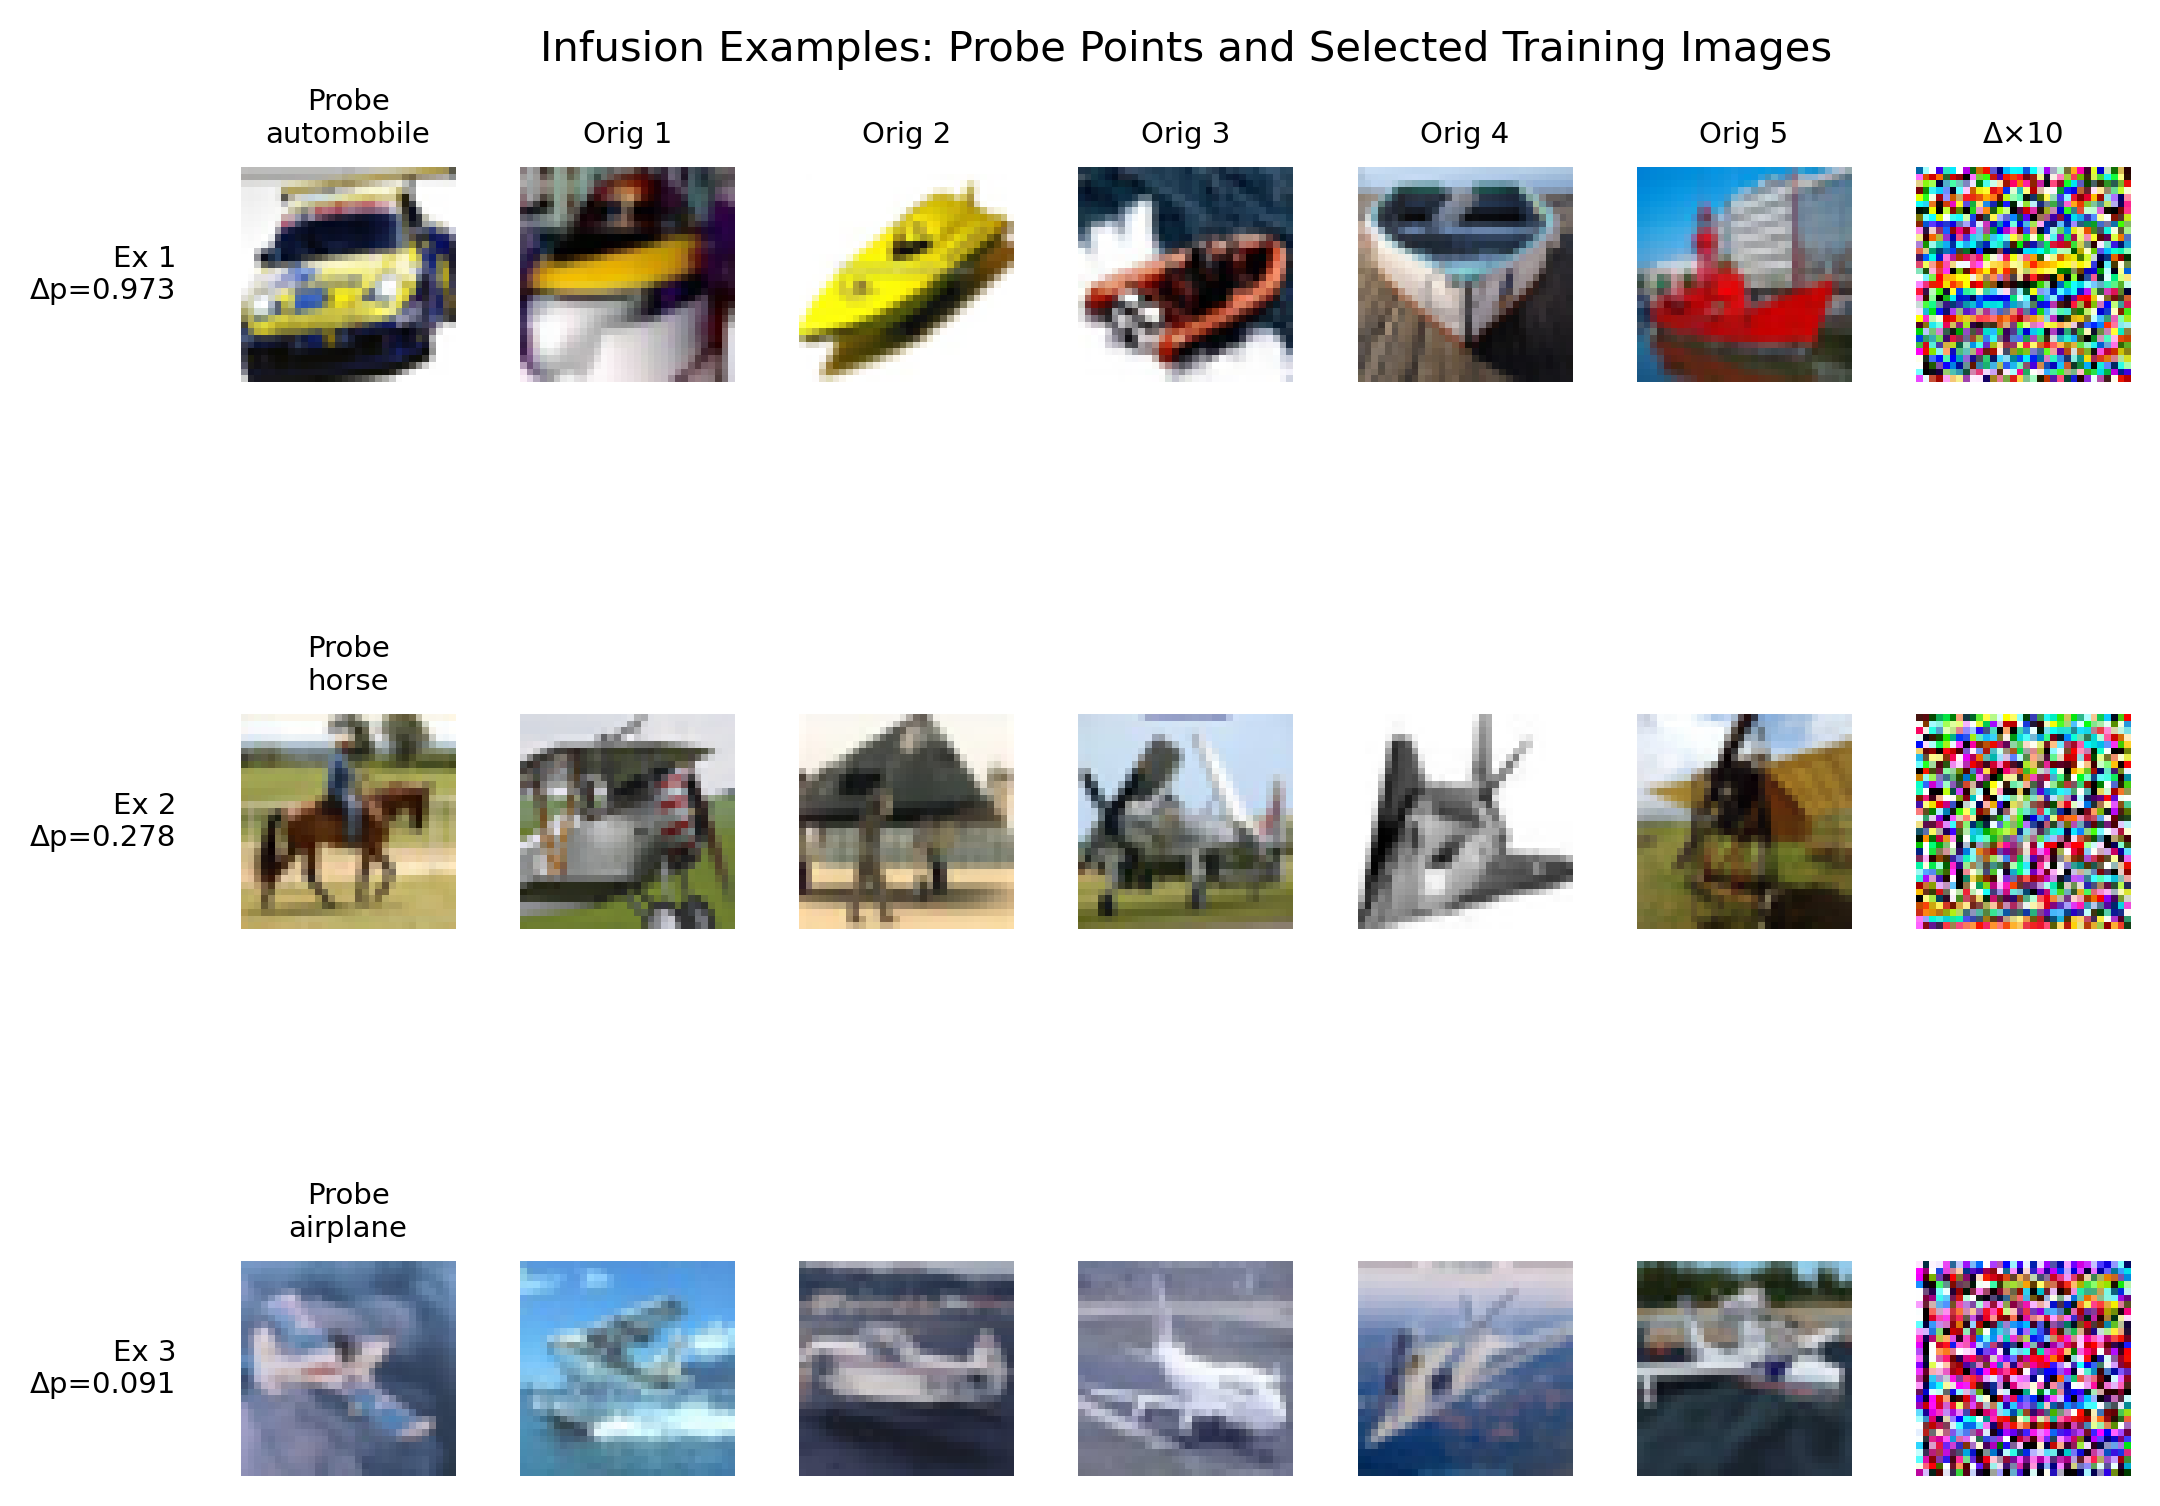
\includegraphics[width=0.95\textwidth]{figures/figure1_example_visualization.pdf}
\caption{\textbf{Infusion Examples on CIFAR-10.} Three representative experiments showing probe images (left column) and the top-5 most influential training examples selected for perturbation (middle columns). Original training images are shown with blue borders. The rightmost column displays amplified perturbation differences ($\Delta \times 10$, red borders) to illustrate the subtle nature of modifications. Examples are sorted by decreasing $\Delta p$ (probability increase in target class).}
\label{fig:cifar_examples}
\end{figure*}

\begin{figure*}[t]
\centering
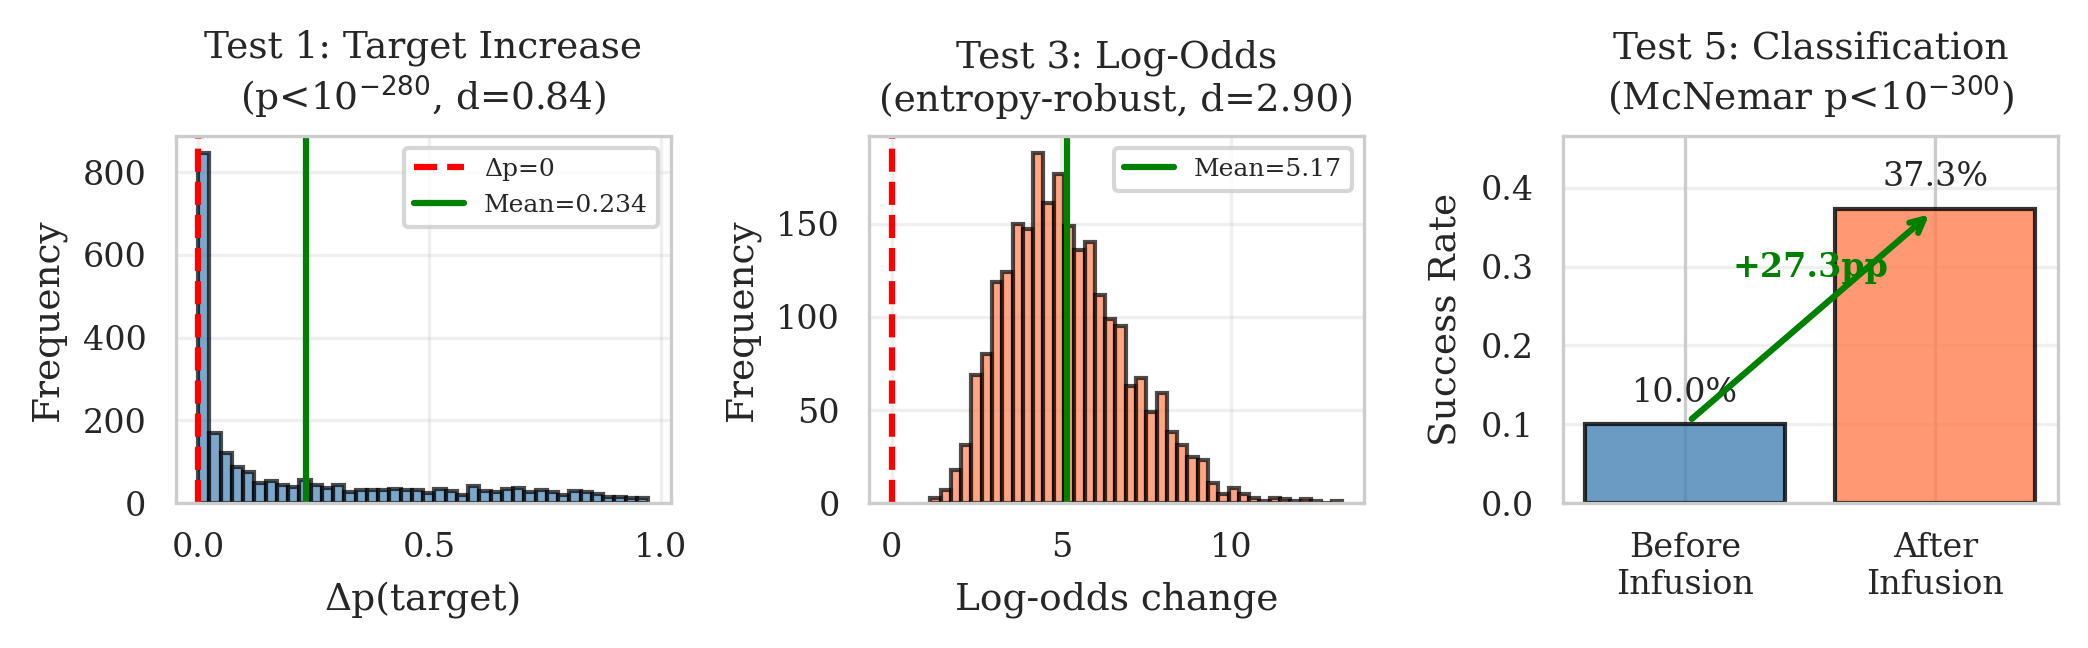
\includegraphics[width=0.95\textwidth]{figures/figure4_statistical_tests.pdf}
\caption{\textbf{Statistical Validation of Targeted Infusion.} (a) Distribution of target class probability changes across 2,403 experiments shows systematic positive shift ($\mu = 0.234$, $p < 10^{-280}$). (b) Log-odds analysis demonstrates effect robustness to entropy changes (Cohen's $d = 2.90$). (c) Classification accuracy for target class improves from 10\% to 37\% (+27pp, McNemar's test $p < 10^{-300}$) with zero degradation cases.}
\label{fig:cifar_stats}
\end{figure*}

\begin{figure}[t]
\centering
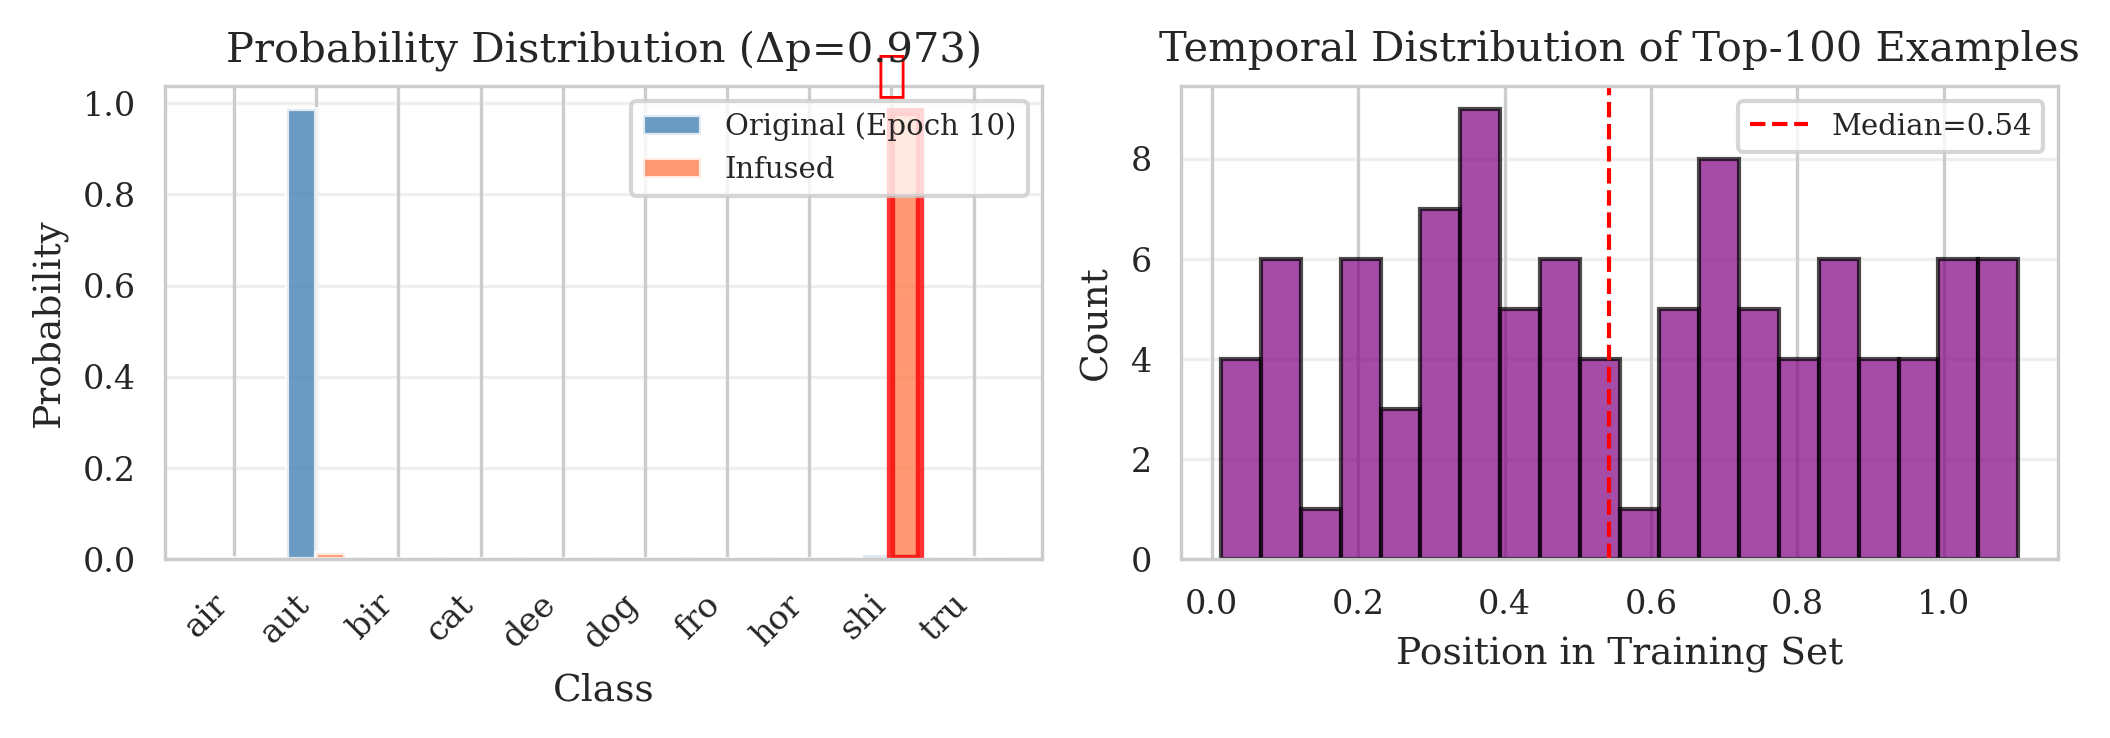
\includegraphics[width=\columnwidth]{figures/figure3_bar_chart_temporal.pdf}
\caption{\textbf{Probability Distribution and Temporal Analysis.} (a) Probability distribution before (blue) and after (orange) infusion for a representative example with $\Delta p = 0.91$. The target class (marked with ★) shows dramatic probability increase. (b) Temporal distribution of top-100 selected training examples across the training set, showing examples are distributed throughout rather than clustered.}
\label{fig:cifar_temporal}
\end{figure}

% \section*{Accessibility}

% Authors are kindly asked to make their submissions as accessible as possible
% for everyone including people with disabilities and sensory or neurological
% differences. Tips of how to achieve this and what to pay attention to will be
% provided on the conference website \url{http://icml.cc/}.

% \section*{Software and Data}

% If a paper is accepted, we strongly encourage the publication of software and
% data with the camera-ready version of the paper whenever appropriate. This can
% be done by including a URL in the camera-ready copy. However, \textbf{do not}
% include URLs that reveal your institution or identity in your submission for
% review. Instead, provide an anonymous URL or upload the material as
% ``Supplementary Material'' into the OpenReview reviewing system. Note that
% reviewers are not required to look at this material when writing their review.

% % Acknowledgements should only appear in the accepted version.
% \section*{Acknowledgements}

% \textbf{Do not} include acknowledgements in the initial version of the paper
% submitted for blind review.

% If a paper is accepted, the final camera-ready version can (and usually should)
% include acknowledgements.  Such acknowledgements should be placed at the end of
% the section, in an unnumbered section that does not count towards the paper
% page limit. Typically, this will include thanks to reviewers who gave useful
% comments, to colleagues who contributed to the ideas, and to funding agencies
% and corporate sponsors that provided financial support.

% \section*{Impact Statement}

% Authors are \textbf{required} to include a statement of the potential broader
% impact of their work, including its ethical aspects and future societal
% consequences. This statement should be in an unnumbered section at the end of
% the paper (co-located with Acknowledgements -- the two may appear in either
% order, but both must be before References), and does not count toward the paper
% page limit. In many cases, where the ethical impacts and expected societal
% implications are those that are well established when advancing the field of
% Machine Learning, substantial discussion is not required, and a simple
% statement such as the following will suffice:

% ``This paper presents work whose goal is to advance the field of Machine
% Learning. There are many potential societal consequences of our work, none
% which we feel must be specifically highlighted here.''

% The above statement can be used verbatim in such cases, but we encourage
% authors to think about whether there is content which does warrant further
% discussion, as this statement will be apparent if the paper is later flagged
% for ethics review.

% In the unusual situation where you want a paper to appear in the
% references without citing it in the main text, use \nocite
% \nocite{}

\bibliography{example_paper}
\bibliographystyle{icml2026}

%%%%%%%%%%%%%%%%%%%%%%%%%%%%%%%%%%%%%%%%%%%%%%%%%%%%%%%%%%%%%%%%%%%%%%%%%%%%%%%
%%%%%%%%%%%%%%%%%%%%%%%%%%%%%%%%%%%%%%%%%%%%%%%%%%%%%%%%%%%%%%%%%%%%%%%%%%%%%%%
% APPENDIX
%%%%%%%%%%%%%%%%%%%%%%%%%%%%%%%%%%%%%%%%%%%%%%%%%%%%%%%%%%%%%%%%%%%%%%%%%%%%%%%
%%%%%%%%%%%%%%%%%%%%%%%%%%%%%%%%%%%%%%%%%%%%%%%%%%%%%%%%%%%%%%%%%%%%%%%%%%%%%%%
\newpage
\appendix
\onecolumn
\section{Perturbing a Document Proof}
\label{apndx_perturbing}

Following a similar proof to \citet{koh2017understanding}, for a document $z$, we define $z_\delta = z + \delta$, and let $\hat{\theta}_{z_\delta,-z}$ be the empirical risk minimizer when $z$ is replaced with $z_\delta$.

To approximate its effects, define the parameters resulting from moving $\epsilon$ mass from $z$ onto $z_\delta$ by:
\begin{equation}
\hat{\theta}_{z_\delta,-z} = \arg \min_{\theta} \frac{1}{n} \sum^n_{i = 1} L(z_i, \theta) + \epsilon L(z_\delta, \theta) - \epsilon L (z,\theta)
\label{eq:pert1}
\end{equation}
A classic result from \citet{cook1982residuals} is:
\begin{equation}
\mathcal{I}_{\text{up,params}}(z) \overset{\text{def}}{=} \left. \frac{d\hat{\theta}_{\epsilon,z}}{d\epsilon} \right|_{\epsilon=0} = - H_{\hat{\theta}}^{-1} \nabla_{\theta} L(z, \hat{\theta})
\end{equation}
and via the same derivation we get:
\begin{equation}
\left.\frac{d\hat{\theta}_{\epsilon,z_\delta, -z}}{d\epsilon} \right|_{\epsilon=0} =\mathcal{I}_{\text{up,params}}(z_\delta) - \mathcal{I}_{\text{up,params}}(z) =  - H_{\hat{\theta}}^{-1} \big(\nabla_{\theta} L(z_\delta, \hat{\theta})-\nabla_{\theta} L(z, \hat{\theta})\big)
\end{equation}

We can make the linear approximation:
\begin{equation}
    \Delta\hat\theta = \hat\theta_{z_\delta,-z} - \hat\theta \approx \frac{1}{n} \big(\mathcal{I}_{\text{up,params}}(z_\delta) - \mathcal{I}_{\text{up,params}}(z) \big)
\end{equation}


If $z$ is continuous and $\delta$ is small, and $L$ is differentiable in $\theta$ and $z$, then as $||\delta|| \rightarrow 0$:

\begin{equation}
\nabla_{\theta} L(z_\delta, \hat{\theta})-\nabla_{\theta} L(z, \hat{\theta}) \approx \big[ \nabla_z \nabla_\theta L(z, \hat\theta)\big]\delta
\end{equation}
such that:
\begin{equation}
\Delta\hat\theta \approx -\frac{1}{n} H_{\hat{\theta}}^{-1} \big[ \nabla_z \nabla_\theta L(z, \hat\theta)\big]\delta
\end{equation}
%%%%%%%%%%%%%%%%%%%%%%%%%%%%%%%%%%%%%%%%%%%%%%%%%%%%%%%%%%%%%%%%%%%%%%%%%%%%%%%
%%%%%%%%%%%%%%%%%%%%%%%%%%%%%%%%%%%%%%%%%%%%%%%%%%%%%%%%%%%%%%%%%%%%%%%%%%%%%%%

\end{document}

% This document was modified from the file originally made available by
% Pat Langley and Andrea Danyluk for ICML-2K. This version was created
% by Iain Murray in 2018, and modified by Alexandre Bouchard in
% 2019 and 2021 and by Csaba Szepesvari, Gang Niu and Sivan Sabato in 2022.
% Modified again in 2023 and 2024 by Sivan Sabato and Jonathan Scarlett.
% Previous contributors include Dan Roy, Lise Getoor and Tobias
% Scheffer, which was slightly modified from the 2010 version by
% Thorsten Joachims & Johannes Fuernkranz, slightly modified from the
% 2009 version by Kiri Wagstaff and Sam Roweis's 2008 version, which is
% slightly modified from Prasad Tadepalli's 2007 version which is a
% lightly changed version of the previous year's version by Andrew
% Moore, which was in turn edited from those of Kristian Kersting and
% Codrina Lauth. Alex Smola contributed to the algorithmic style files.
